
%%%%%%%%%%%%%%%%%%%%%%%%%%%%%%%%%%%%%%%%%%%%%%%%%%%%%%%%%%
\chapter{Qualitative Metrics}
%%%%%%%%%%%%%%%%%%%%%%%%%%%%%%%%%%%%%%%%%%%%%%%%%%%%%%%%%%

\mynote
{
\begin{itemize}
\item adequacy, efficiency, productiveness, effectiveness (choose your criteria, state them clearly and justify them)
\item be careful that you are using a fair measure, and that you are actually measuring what you claim to be measuring
\item if comparing with previous techniques those techniques must be described in Chapter 2
\item be honest in evaluation
\item admit weaknesses
\end{itemize}
}

%%%%%%%%%%%%%%%%%%%%%%%%%%%%%%%%%%%%%%%%%%%%%%%%%%%%%%%%%%
\section{The Overlap Function}
%%%%%%%%%%%%%%%%%%%%%%%%%%%%%%%%%%%%%%%%%%%%%%%%%%%%%%%%%%


%%%%%%%%%%%%%%%%%%%%%%%%%%%%%%%%%%%%%%%%%%%%%%%%%%%%%%%%%%
\section{Spherical Contact Probability}
%%%%%%%%%%%%%%%%%%%%%%%%%%%%%%%%%%%%%%%%%%%%%%%%%%%%%%%%%%


%%%%%%%%%%%%%%%%%%%%%%%%%%%%%%%%%%%%%%%%%%%%%%%%%%%%%%%%%%
\section{Histograms of the Distance Transform}
%%%%%%%%%%%%%%%%%%%%%%%%%%%%%%%%%%%%%%%%%%%%%%%%%%%%%%%%%%


%%%%%%%%%%%%%%%%%%%%%%%%%%%%%%%%%%%%%%%%%%%%%%%%%%%%%%%%%%
\section{Comparisons}
%%%%%%%%%%%%%%%%%%%%%%%%%%%%%%%%%%%%%%%%%%%%%%%%%%%%%%%%%%


\begin{figure}
\centering
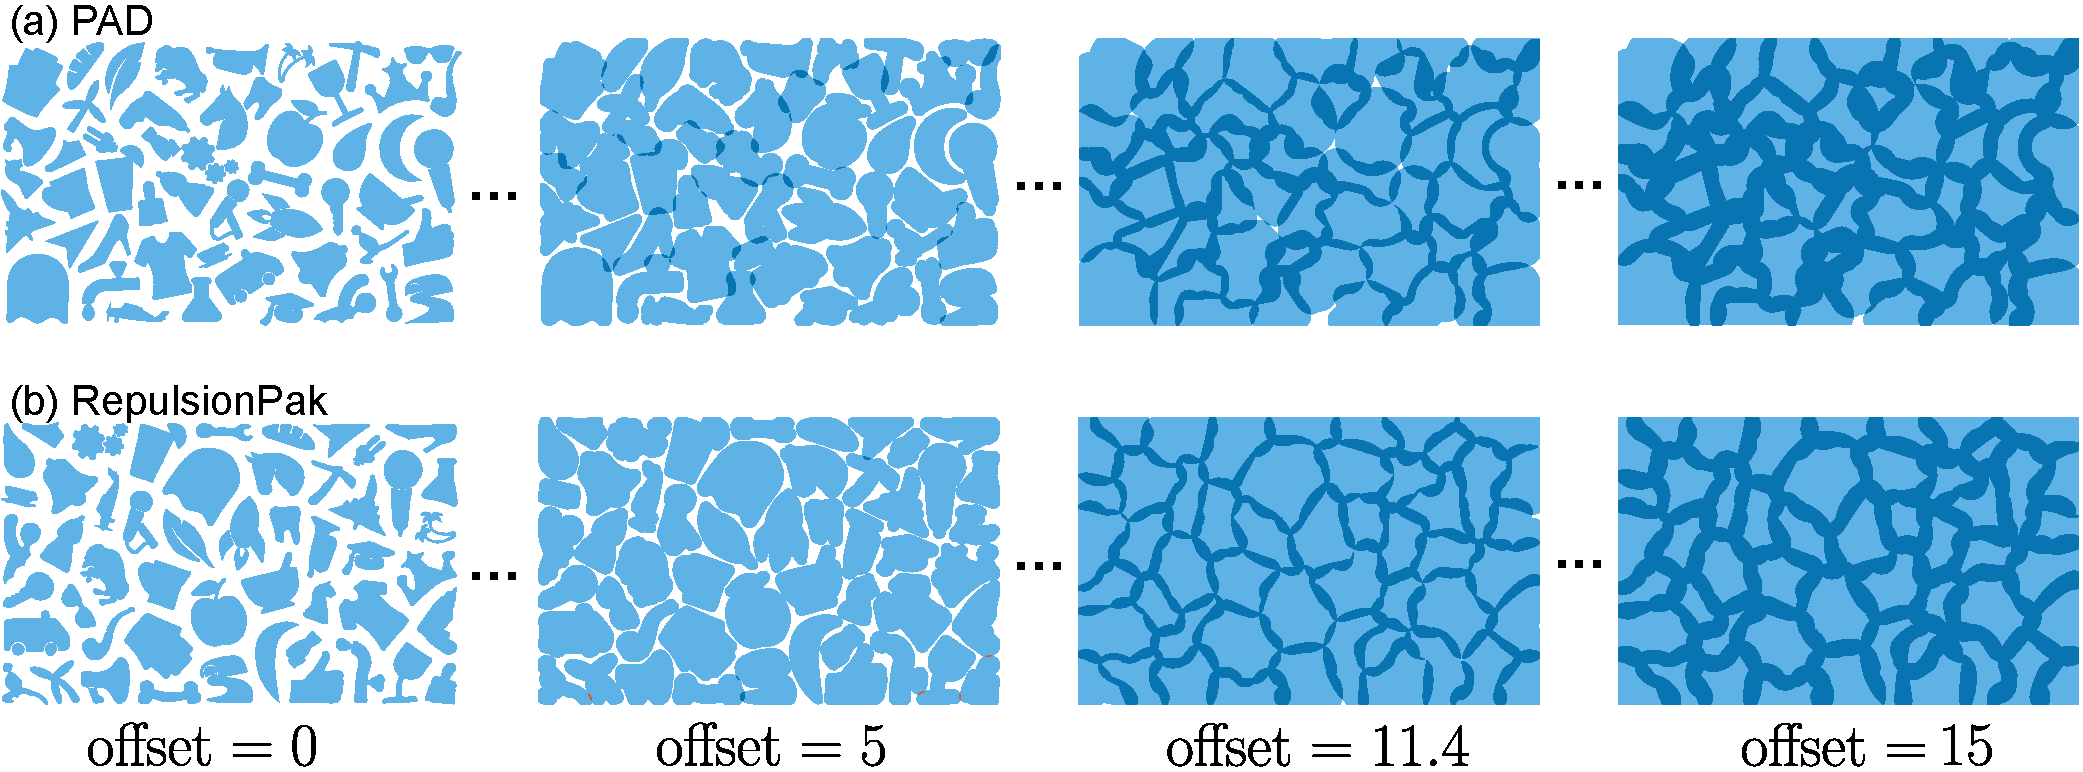
\includegraphics[width=1.0\textwidth]{figures/metrics/overlap_metric.pdf}
\caption[An illustration of offsetting elements outward]
{\label{fig_overlap_function}
    An illustration of offsetting elements outward. The packings have $d_\mathrm{gap} / 2 = 5.7$.  
    At an offset of 5, which is slightly less than $d_\mathrm{gap} / 2$,
    the overlap for the PAD packing is 1.462\% of the total area, while the overlap for our packing is only 0.039\%.
    At an offset of 11.4, which equals $d_\mathrm{gap}$, the PAD packing shows more empty space (1.05\%) than RepulsionPak (0.07\%).
    As the offset is increased, overlaps in the PAD packing create channels
  with uneven widths, whereas ours are more uniform.
  }
\end{figure}

\begin{figure}
\centering
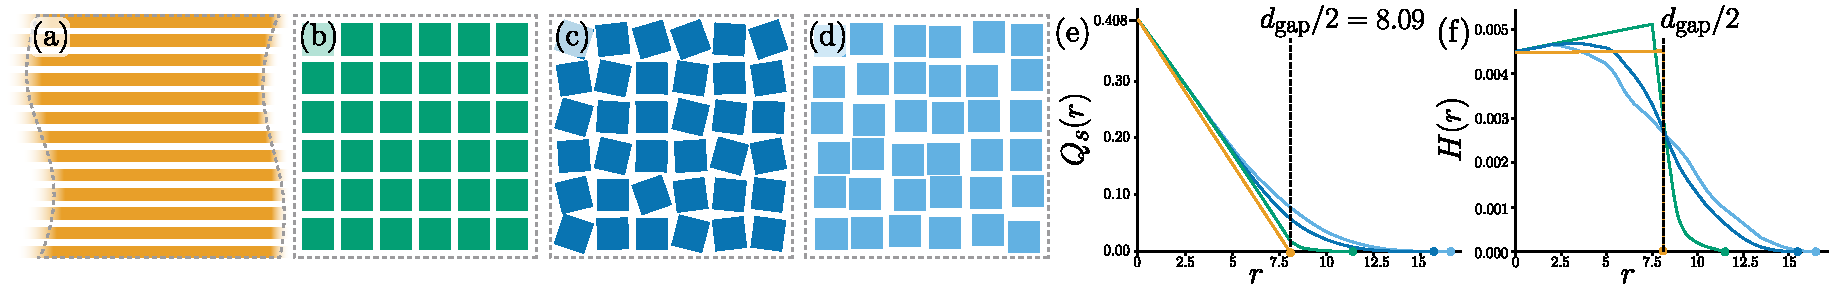
\includegraphics[width=1.0\textwidth]{figures/metrics/hsr_viz.pdf}
\caption[Spherical contact probabilities and distance histograms \newline for reference packings]
{\label{hsr_viz}
Spherical contact probabilities and distance histograms for 
reference packings.
A ``perfect packing'' of infinite stripes is shown in~(a),
followed by a square packing with the same area fraction and $d_\mathrm{gap}$
in~(b).  The square packing is then perturbed with random rotations in~(c)
and translations in~(d). The corresponding SCP functions and histograms are plotted
in~(e) and~(f).}
\end{figure}

\begin{figure}
\centering
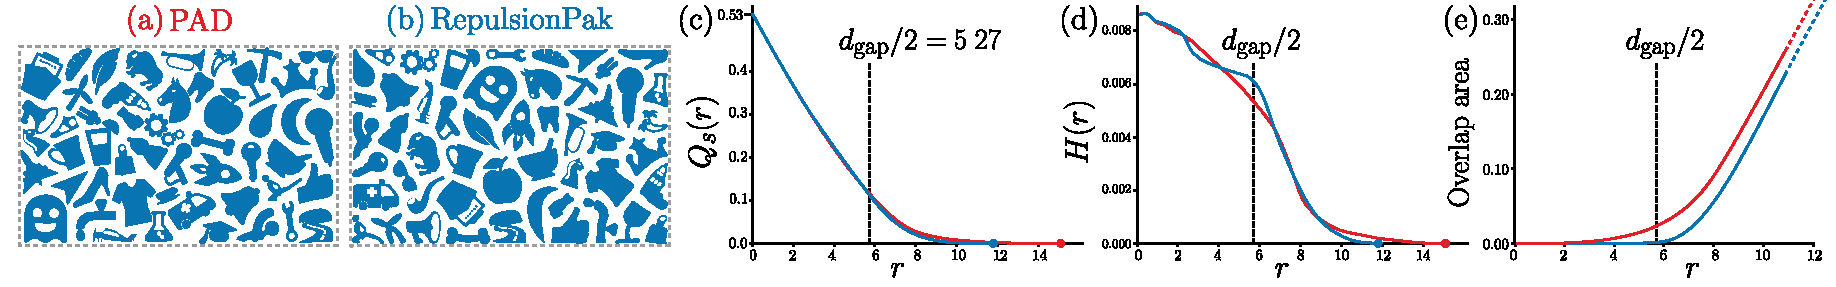
\includegraphics[width=1.0\textwidth]{figures/metrics/pad_comparison.pdf}
\caption[A comparison between a PAD~packing and a RepulsionPak packing \newline  with their corresponding SCPs]
{\label{pad_comparison}
    A comparison between a PAD~packing shown in~(a) and a RepulsionPak packing in~(b) 
    with their corresponding SCPs~(c), distance histograms~(d), and overlap functions~(e). 
  The PAD and RepulsionPak packings are calibrated
  to have the same negative space ratio.
    Our SCP is lower and shorter than the PAD's result,
    our histogram shows higher concentration around $d_\mathrm{gap} / 2$,
    indicating more even negative space,
    and our packing has a lower overlap function.
}
\end{figure}

\begin{figure}
\centering
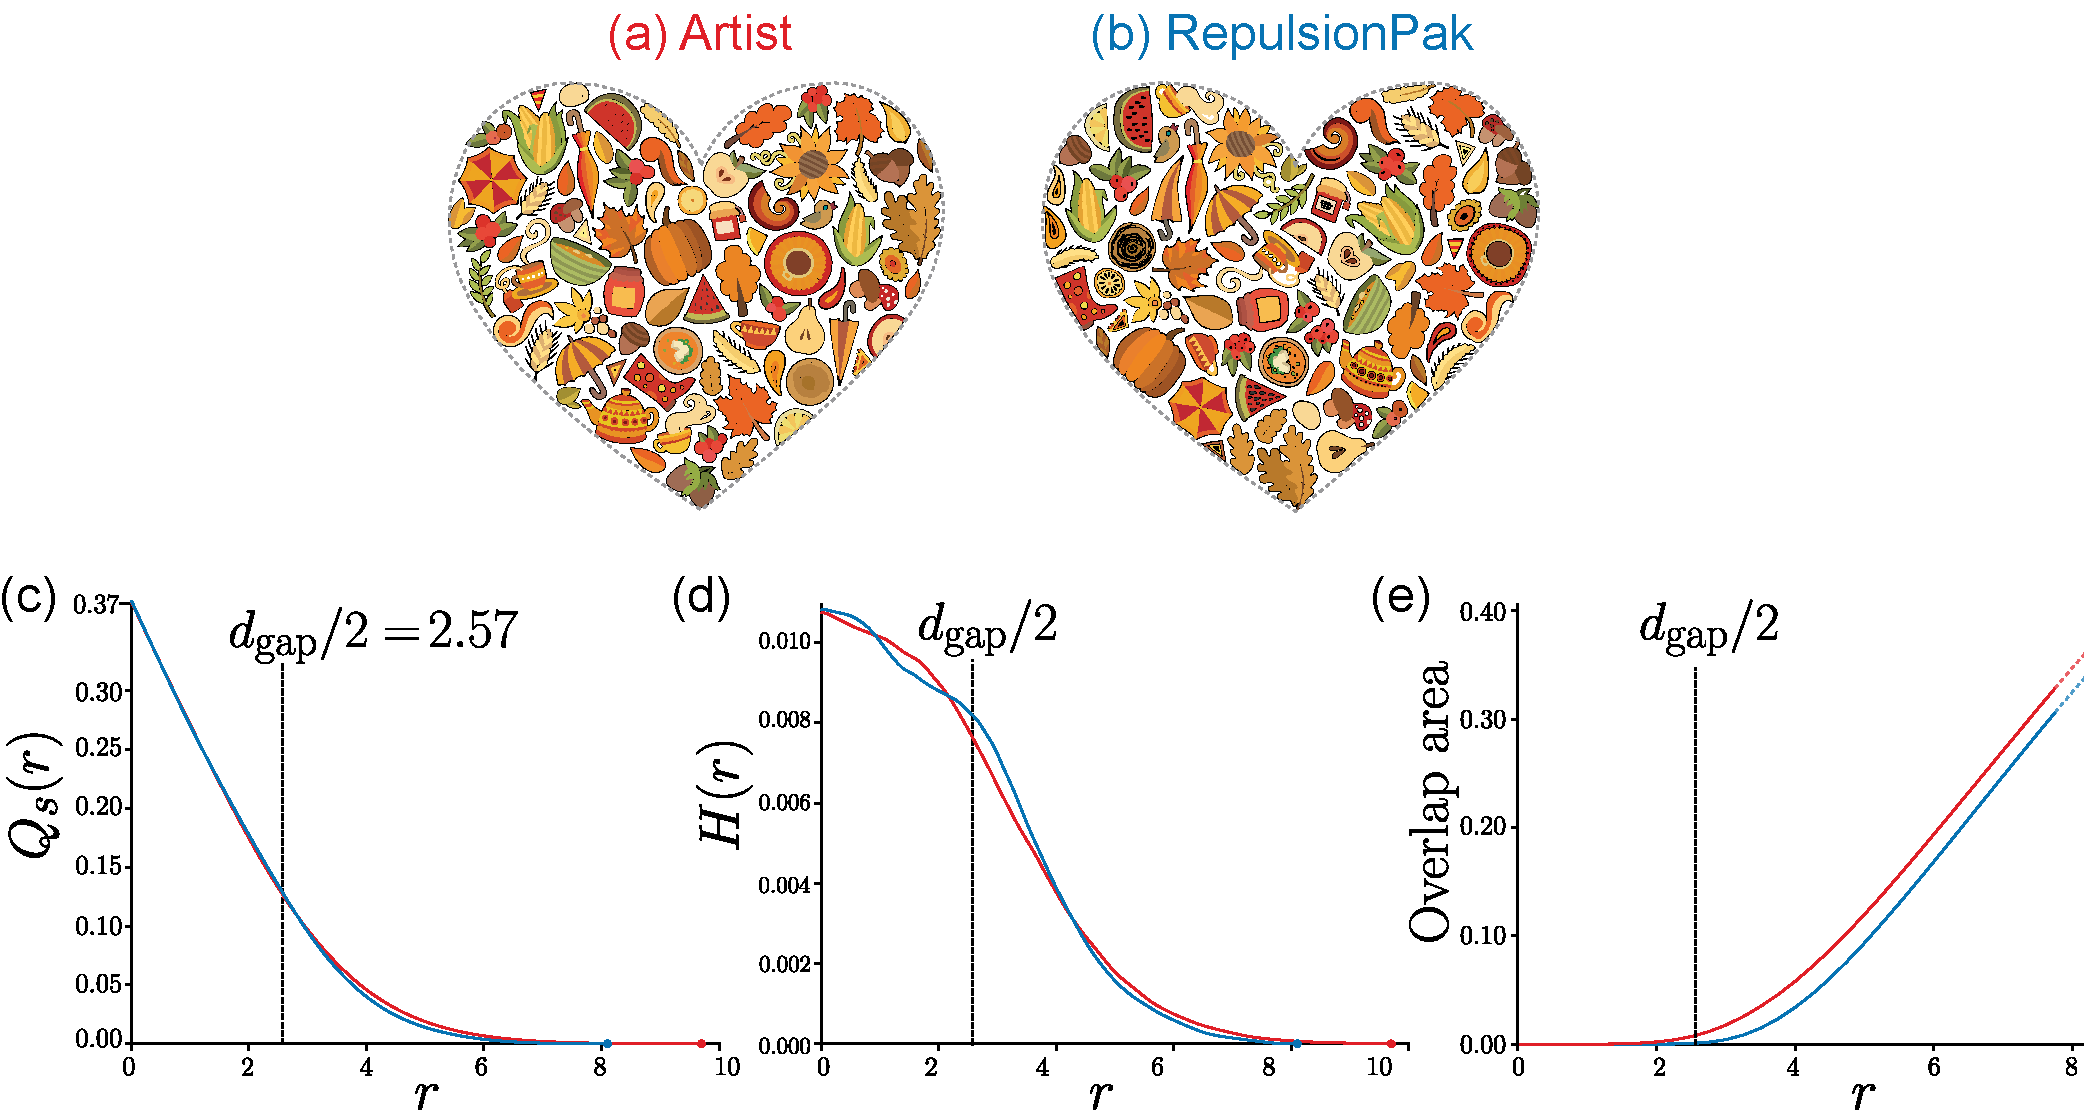
\includegraphics[width=1.0\textwidth]{figures/metrics/balabolka_comparison.pdf}
\caption[A comparison between the artist-made packing \newline  and a RepulsionPak packing]
{ \label{balabolka_comparison} 
    A comparison between the artist-made packing from 
  Fig.~\ref{packing_example}, shown in~(a), and a RepulsionPak packing
  with the same elements in~(b).  We plot the corresponding SCPs~(c),
  distance histograms~(d), and overlap functions~(e).
    For comparison purposes we remove secondary elements from the artist's
  packing.  Our SCP is lower and shorter than the artist's result,
    our histogram shows more concentration around $d_\mathrm{gap} / 2$,
    and RepulsionPak also has a lower overlap function.
}
\end{figure}

\begin{figure}
\centering
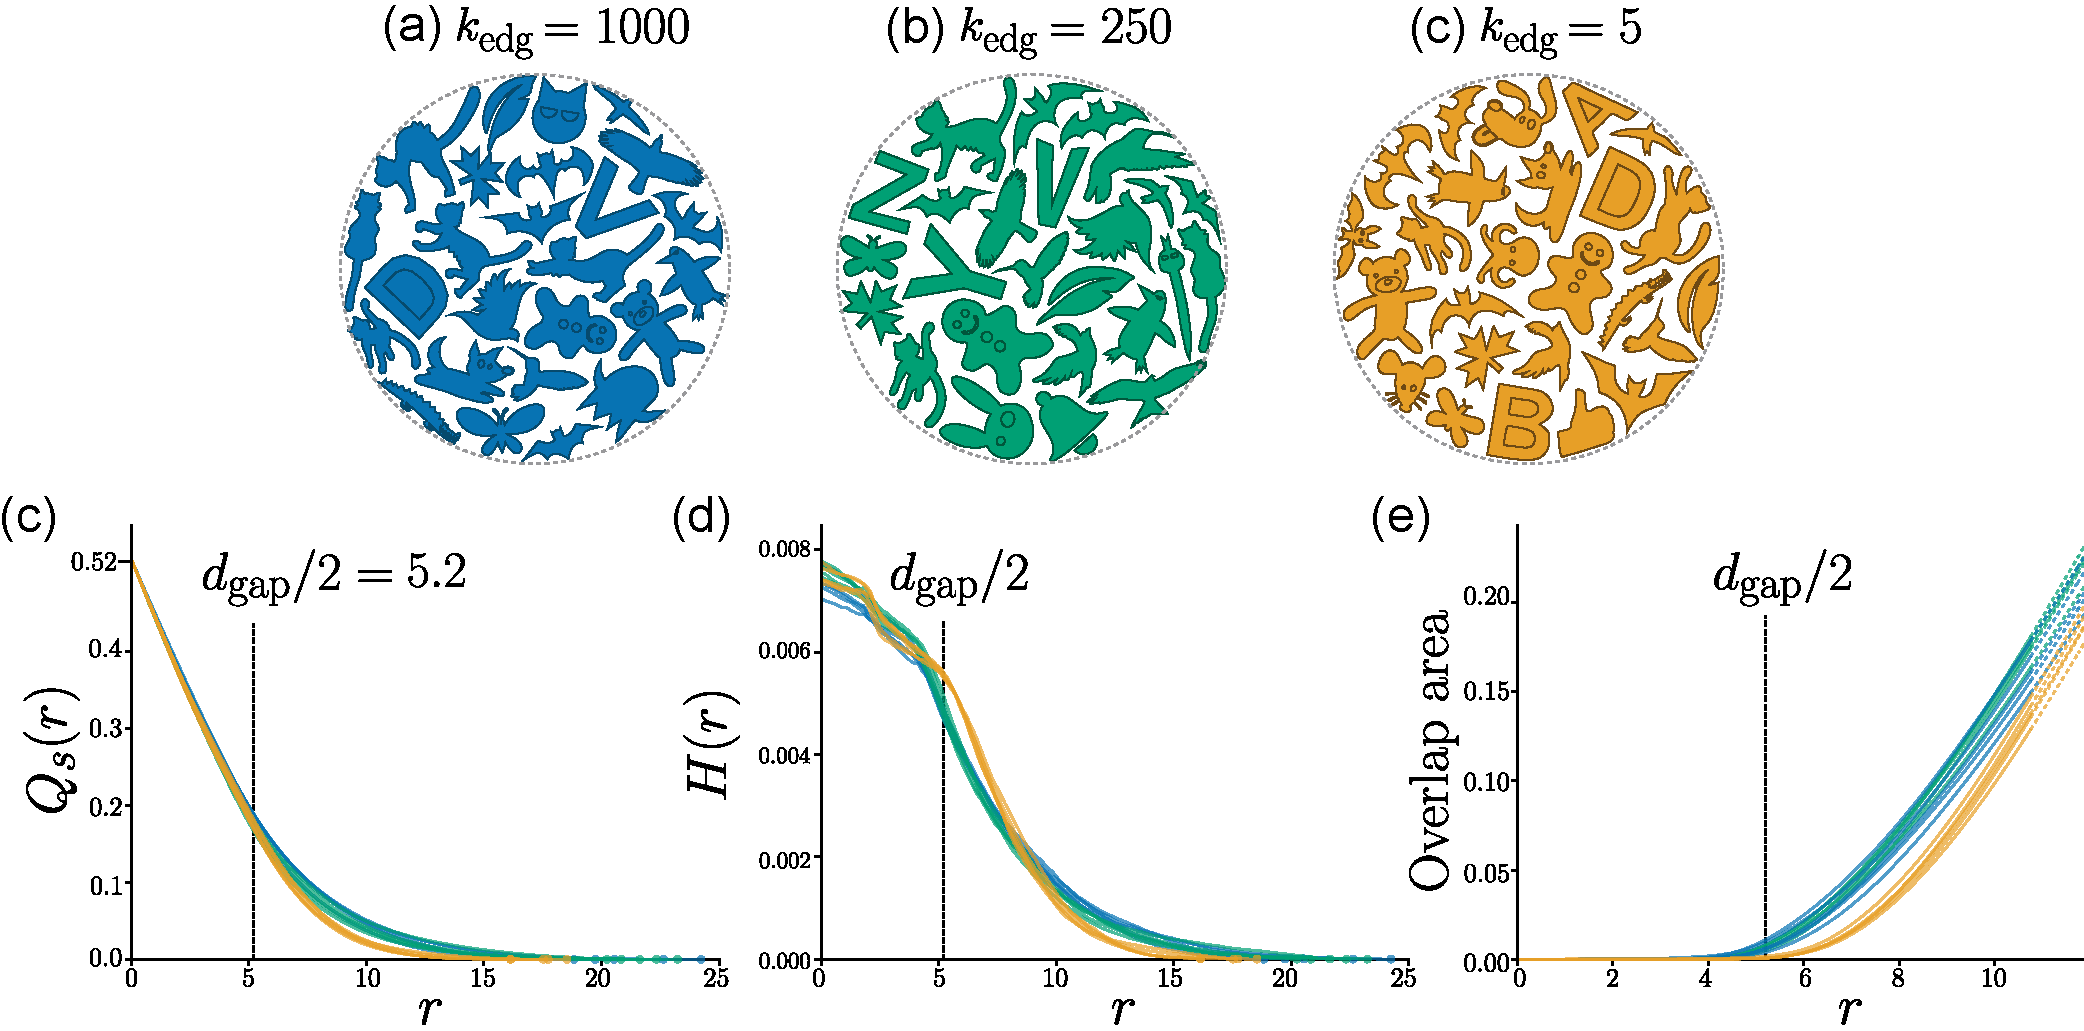
\includegraphics[width=1.0\textwidth]{figures/metrics/evaluation.pdf}
\caption[A demonstration of the effect of deformation \newline on the evenness of negative space]
{\label{fifteen_packings}
    A demonstration of the effect of deformation on the evenness of negative space.  
    The packings in (a), (b) and (c) are representative results using three values of the edge force strength $k_e$,
    from 
	rigid ($k_e=1000$) to moderate ($k_e=250$) to deformable ($k_e=5$).
% 	deformable ($k_e=5$) to moderate ($k_e=250$) to rigid ($k_e=1000$).
	We construct
    five random packings for each value of $k_e$, and plot their SCPs~(d), histograms~(e), and overlap functions~(f).
    Packings with the most deformation have steeper and shorter SCPs, 
    more histogram concentrations around $d_\mathrm{gap} / 2$, and lower overlap functions.
}
\end{figure}